\documentclass[a4paper]{book}

\usepackage[spanish]{babel}
\usepackage[utf8]{inputenc}

\usepackage[backend=biber]{biblatex}
% \usepackage{amsmath}
% \usepackage{amsfonts}
% \usepackage{amssymb}
% \usepackage{amsthm}
% \usepackage{enumerate}
% \usepackage{color}
% \usepackage{graphicx}
\usepackage{todonotes}
\usepackage[hidelinks]{hyperref}

\newcommand{\todoGuido}[1]{\todo[color=red]{Guido: {#1}}}
\newcommand{\todoCarlos}[1]{\todo[color=green]{Carlos: {#1}}}

\addbibresource{referencias.bib}
\setcounter{tocdepth}{1}

\begin{document}

%%%% Title Page
\begin{titlepage}

\newcommand{\HRule}{\rule{\linewidth}{0.5mm}}  % horizontal line and its thickness

\center

% University
\textsc{\LARGE Universidad Nacional de Rosario} \\[1cm]

% Document info
\textsc{\Large Tesina de grado}\\[0.1cm]
\textsc{\large para la obtención del grado de}\\[0.1cm]
\textsc{\large Licenciado en Ciencias de la Computación}\\[1cm]

\HRule \\[0.8cm]
{\Large \bfseries Hacia un prototipo certificado del sistema de seguridad de
Android~9 }\\[0.7cm]        % Assignment
\HRule \\[2cm]


\large

\includegraphics[width=0.3\textwidth]{imagenes/unr.jpg}\\[3cm] 	% University logo
\emph{Alumno:}\\
Guido De Luca \\[1.5cm]
{\large \today}\\[2cm]
\vfill
\end{titlepage}

\tableofcontents



\chapter{Estado del arte}
\label{chapter:estado}

En esta sección se presentan algunos trabajos académicos relacionados con el
modelo de seguridad de Android. Se organizará de la siguiente manera: primero,
se describen trabajos informales\footnote{Entendemos por trabajo informal a
aquellos que describen coloquialmente el sistema, por más rigurosa que sea la
descripción} que son de interés por abarcar características nuevas, por la
información que condensan o por ser pioneros en el área. Luego, se mencionan
varias herramientas (o aplicaciones) que utilizan técnicas de análisis estático
de código para detectar potenciales vulnerabilidades, todas desarrolladas dentro
de un marco académico. A pesar de que este enfoque  es distinto al que se
propone en esta tesina, se tomó la decisión de incluirlo en este capítulo ya que
conforma gran parte de la investigación actual y de los últimos años. Por
último, se analizan aquellos trabajos que utilizan métodos formales para dar una
especificación de la plataforma. Estos trabajos se describen con más detalle que
los anteriores e incluso se contemplan artículos que no son recientes pero
presentan un enfoque novedoso o relevante a este trabajo.

Dentro del primer grupo, se encuentran artículos como el de William Enck
\textit{et al.}~\cite{enck}: uno de los primeros trabajos académicos en
describir el modelo de seguridad de Android. Los autores buscaban
\textit{desenmascarar} la complejidad a la que debían enfrentarse los
desarrolladores cuando se proponían construir aplicaciones seguras. A pesar de
la antigüedad de este artículo, hoy en día sigue siendo relevante por la
explicación concreta y concisa sobre las bases del sistema de permisos de
Android. También se encuentra el trabajo de Wang y Wu~\cite{wang}, quienes
resumen las vulnerabilidades que existen en el sistema de comunicación entre
componentes, para luego discutir sobre el estado del arte en la detección y
prevención de las mismas.

Recientemente, René Mayrhofer \textit{et al.}~\cite{mayrhofer} realizaron un
trabajo similar para la versión 9.0 de Android. En él, se definen los principios
de seguridad del sistema en cuestión y un modelo de amenazas \textit{por capas},
a partir cual se derivan amenazas concretas que dependen de la cercanía entre
atacante y dispositivo móvil. Además, este artículo analiza los cambios que se
fueron introduciento en el sistema operativo para mitigar estas amenazas.

% Por otro lado, tenemos el trabajo de Yasemin Acar \textit{et al.}~\cite{sok},
% quienes presentan una visión sistémica e integradora de las distintas líneas
% de investigación en Android. Los autores realizan un análisis de los diversos
% enfoques desde los cuales se aborda la seguridad de esta plataforma,
% comparándolos, y estableciendo, según ellos, cuál es el camino para la
% investigación futura.

Este tipo de trabajos constituyen un complemento importante a la documentación
oficial de Android, brindándole referencias más claras a los desarrolladores y
nuevas herramientas que permiten resguardar sus aplicaciones. Un ejemplo de esto
fue el trabajo de Felt \textit{et al.}~\cite{felt}, quienes estudiaron un grupo
de aplicaciones disponibles para la versión 2.2 de Android y detectaron que
muchas de ellas pedían más permisos de los que realmente necesitaban. Los
autores investigaron las causas de sobreprivilegio de estas aplicaciones y
encontraron que, muchas veces, los desarrolladores intentaban otorgar la menor
cantidad de privilegios necesarios, pero en reiteradas ocasiones fallaban por
falta de una documentación precisa. En consecuencia, el grupo desarrolló
Stowaway, una de las primeras herramientas dedicadas a la detección de permisos
innecesarios.

Actualmente existe una gran cantidad de herramientas de análisis estático que
ayudan a detectar sobreprivilegios o un flujo de información indebido, siendo
las más recientes:
%
M-Perm~\cite{mperm},
%
IC3~\cite{ic3},
% que incorpora el concepto de \textit{propagación de constantes compuestas
% multi-valuadas} para lograr una mayor eficiencia;
Droidtector~\cite{droidtector},
% que a diferencia del resto no necesita el código fuente de las aplicaciones o
% de Android para realizar el análisis.
Covert~\cite{covert} y Separ~\cite{separ}.
% que combinan análisis estático con métodos formales para inferir
% automáticamente propiedades sobre un conjunto de aplicaciones, a partir de las
% cuales se derivarán políticas de seguridad
Las dos últimas combinan análisis estático con métodos formales para inferir
automáticamente propiedades sobre un conjunto de aplicaciones y luego derivar
políticas de seguridad. La gran oferta que existe de este tipo de aplicaciones,
da lugar a trabajos como el Lina Qiu \textit{et al.}~\cite{qiu}, en el que se
analizan y comparan las herramientas, que según los autores, son las más
destacadas: Flowdroid combinada con IccTA~\cite{iccta},
Amandroid~\cite{amandroid} y DroidSafe~\cite{droidsafe}.

Abordar la seguridad de Android con este enfoque presenta una diferencia
fundamental con respecto a la que se propone en esta tesina: estas herramientas
se focalizan en proteger una aplicación en particular (o en algunos casos, un
conjunto de aplicaciones); mientras que una especificación formal de la
plataforma subyacente permite extraer propiedades relevantes a \textbf{todas}
las aplicaciones y al sistema en general. Por otro lado, este tipo de
aplicaciones son un recurso más accesible para los usuarios que desean
resguardar información sensible sin ser especialistas en el área.

% A pesar de ser el enfoque con más publicaciones relacionadas a la seguridad de
% Android, presenta una diferencia fundamental con el que se propone en esta
% tesina: estas herramientas se focalizan en estudidar una aplicación (o en
% algunos casos, un conjunto de aplicaciones)


% Las herramientas e este tipo se focalizan en estudiar una aplicación en
% particular (o en algunos casos, un conjunto de aplicaciones) y extraer
% propiedades de seguridad que solo conciernen a ella. En cambio, en esta tesina
% estudiamos el sistema de permisos subyacente, extrayendo propiedades
% relevantes para todas las aplicaciones y para el sistema en general.


Entrando en el terreno de los métodos formales, nos encontramos en primer lugar
con el trabajo de Chaudhuri~\cite{chaudhuri}. En el mismo, se desarrolló un
lenguaje que permite describir un subconjunto de aplicaciones de Android y
razonar sobre ellas. Adicionalmente, se presentó un sistema de tipos para este
lenguaje y se demostró un teorema que garantiza que las aplicaciones bien
tipadas preservan la confidencialidad de los datos que manejan. Parcialmente
inspirado en este trabajo, Bugliesi \textit{et al.} desarrollaron
$\pi$-Perm~\cite{bugliesi}, un sistema de tipos y efectos que tiene como
finalidad detectar problemas de \textit{privilege escalation}. De manera análoga
al trabajo de Chaudhuri, una expresión bien tipada en $\pi$-Perm garantiza que
la aplicación real a la cual está representando, no es vulnerable al ataque
mencionado. Similarmente, Armando \textit{et al.} definen un
lenguaje~\cite{armando}, acompañado por su semántica operacional, que permite
describir interacciones entre aplicaciones. Al igual que en los trabajos
anteriores, se define un sistema de tipos y efectos; pero este está basado en un
formalismo del estilo del álgebra de procesos, conocido como \textit{history
expressions}~\cite{history-expressions}. Puesto en términos simples, una
\textit{history expression} sirve para representar los efectos laterales
vinculados a la seguridad del dispositivo, que se producen al realizar una
computación. Finalmente, los autores prueban que cualquier comportamiento que la
plataforma pueda tener en \textit{runtime}, está contenido en este modelo; y por
lo tanto, puede analizarse estáticamente.

Recientemente, Wilayat Khan \textit{et al.}~\cite{khan} retomaron el trabajo de
Chaudhuri y modelaron el lenguaje en él definido dentro del \textit{framework}
lógico-matemático Coq~\cite{coq}. De esta forma, pudieron no solo estudiar la
corrección y seguridad de las aplicaciones de manera mecánica y rigurosa, sino
que también utilizaron este asistente para probar la corrección -o
\textit{soundness}- del lenguaje en sí. En otro trabajo actual en el que
participó Khan~\cite{crashsafe}, se definió en Coq un modelo para estudiar el
sistema de comunicación entre componentes. El principal objetivo de este trabajo
es analizar la robustez de la plataforma cuando una aplicación detiene su
ejecución a causa de un fallo en la resolución de un \textit{intent}. A
diferencia del resto de los trabajos citados, éste se concentra en estudiar
propiedades de \textit{safety} y no de \textit{security}, a pesar de que este
sistema puede ser explotado para filtrar información sensible de los
usuarios~\cite{iccta}.

Por otra parte, Sadeghi \textit{et al.}~\cite{sadeghi-temp} presentan una
formalización de la plataforma escrita en TLA+, un lenguaje especificación
basado en la lógica lineal temporal~\cite{tla+}. Al incoporar el aspecto
temporal al modelo, los autores buscan definir propiedades cuya veracidad
dependa del momento en el que se la evalúe y de esta forma, modelar el
comportamiento del sistema a medida que evoluciona en el tiempo. Luego, proponen
un monitor de seguridad que otorga permisos temporales a las aplicaciones
siempre y cuando se cumplan todas las propiedades (o reglas) de seguridad
previamente definidas. Este permiso ``prestado'' es automáticamente revocado si
en algún momento el sistema se encuentra en un estado que compromete alguna de
las reglas.

Similarmente, Bagheri \textit{et al.}~\cite{bagheri15} proponen una
formalización del sistema de permisos de Android escrita en Alloy~\cite{alloy}:
un lenguaje basado en la lógica relacional de primer orden, que incorpora una
herramienta capaz de realizar análisis de satisfacibilidad automáticos sobre los
modelos en él descriptos. Con la ayuda de esta formalización, los autores
identificaron distintos tipos de vulnerabilidades que permiten esquivar el
chequeo de permisos. Particularmente, estudiaron la vulnerabilidad de permisos
personalizados, mediante la cual una aplicación maliciosa puede acceder a todos
los recursos de otra que estén protegidos por permisos personalizados. Esta
falla surge de que el sistema no impone restricciones con respecto al nombre de
los nuevos permisos que definen y, como consecuencia, dos permisos distintos
podrían tener el mismo nombre. Este trabajo luego se extendió para una nueva
versión de Android~\cite{bagheri}. La falla por permisos personalizados había
sido reportada previamente por Shin \textit{et al.}~\cite{shin-custom}. Una
diferencia fundamental entre este enfoque y el de esta tesina es el tipo de
análisis que se realizó. A pesar de que Alloy es capaz de producir
contraejemplos de manera automática, algo realmente útil a la hora de buscar
potenciales fallas; no es posible demostrar propiedades de una manera rigurosa y
formal.

En trabajos previos encabezados por Gustavo Betarte y Carlos
Luna~\cite{betarte-2017, betarte-2016, luna-cleiej}, se utilizó el asistente de
pruebas Coq para modelar un sistema de transición de estados que representa,
principalmente, los distintos estados que atraviesa la plataforma cuando se
realizan operaciones sobre ella (por ejemplo, al instalar o desinstalar una
aplicación). A partir de esta especificación, no solo se probaron propiedades
relevantes a la seguridad del modelo, sino que también se extrajo una
implementación certificada del mismo. Los autores explican cómo esta
implementación puede utilizarse para generar casos de pruebas abstractos dentro
del \textit{testing} basado en modelos, o bien, cómo puede usarse para
monitorear las acciones realizadas en un sistema real y evaluar si las
propiedades deseadas efectivamente se cumplen. Estos trabajos presentan el
modelo que será actualizado y extendido en esta tesina.

%%%%%%%%%%
% Fragmento tomado de \cite{luna-cleiej}
%%%
% In particular, Shin et al. [42, 43] build a formal framework that represents
% the Android permission system, which is based on the Calculus of Inductive
% Constructions and it is developed in Coq, as we do. However, that
% formalization does not consider, for instance, several aspects of the platform
% covered in our model, namely, the different types of components, the
% interaction between a running instance and the system, the reading/writing
% operation on a content provider and the semantics of the permission delegation
% mechanism. They also do not consider novel aspects of the Android security
% model, such as managing runtime permissions.
%%%
Un enfoque similar a este, es el de Wook Shin \textit{et al.}, quienes también
utilizaron Coq para modelar el sistema de permisos de Android~\cite{shin}. Sin
embargo, esta formalización no considera aspectos de la plataforma que sí son
considerados por los trabajos anteriores (y por ende, por esta tesina); como por
ejemplo, los distintos tipos de componentes, la interacción entre instancias de
aplicaciones en ejecución y el sistema, la operación de escritura/lectura en un
\textit{content provider} y la semántica del sistema de delegación de permisos.
Al mismo tiempo, cuando Android incorporó los permisos otorgados en
\textit{runtime}, este modelo no fue actualizado. El trabajo de Fragkaki \textit{et al.}
tambień presenta un modelo formal basado en transiciones de
estado~\cite{fragkaki}, pero el mismo no está desarrolado dentro de un
\textit{framework} que permita realizar pruebas asisistidas por computadora.
Además, el modelo se corresponde con una de las primeras versiones de Android,
por lo que tampoco contempla los cambios más recientes en el sistema de
permisos.
\chapter{El modelo de seguirdad de Android}
\label{chapter:background}

\section{Arquitectura de la plataforma}
\label{section:architecture}

El sistema operativo Android está compuesto por cinco capas de software, ordenadas en forma de pila
(o \textit{stack}), donde cada una de ellas provee un grupo de servicios a la capa inmediatamente
superior. De esta forma, se va abstrayendo progresivamente la interacción con el hardware (la base
de la pila) hasta llegar al nivel más alto, en el que se ubican las aplicaciones que realizarán las
tareas requeridas por los usuarios. A continuación, analizaremos brevemente cada uno de estos
niveles.

\begin{figure}
    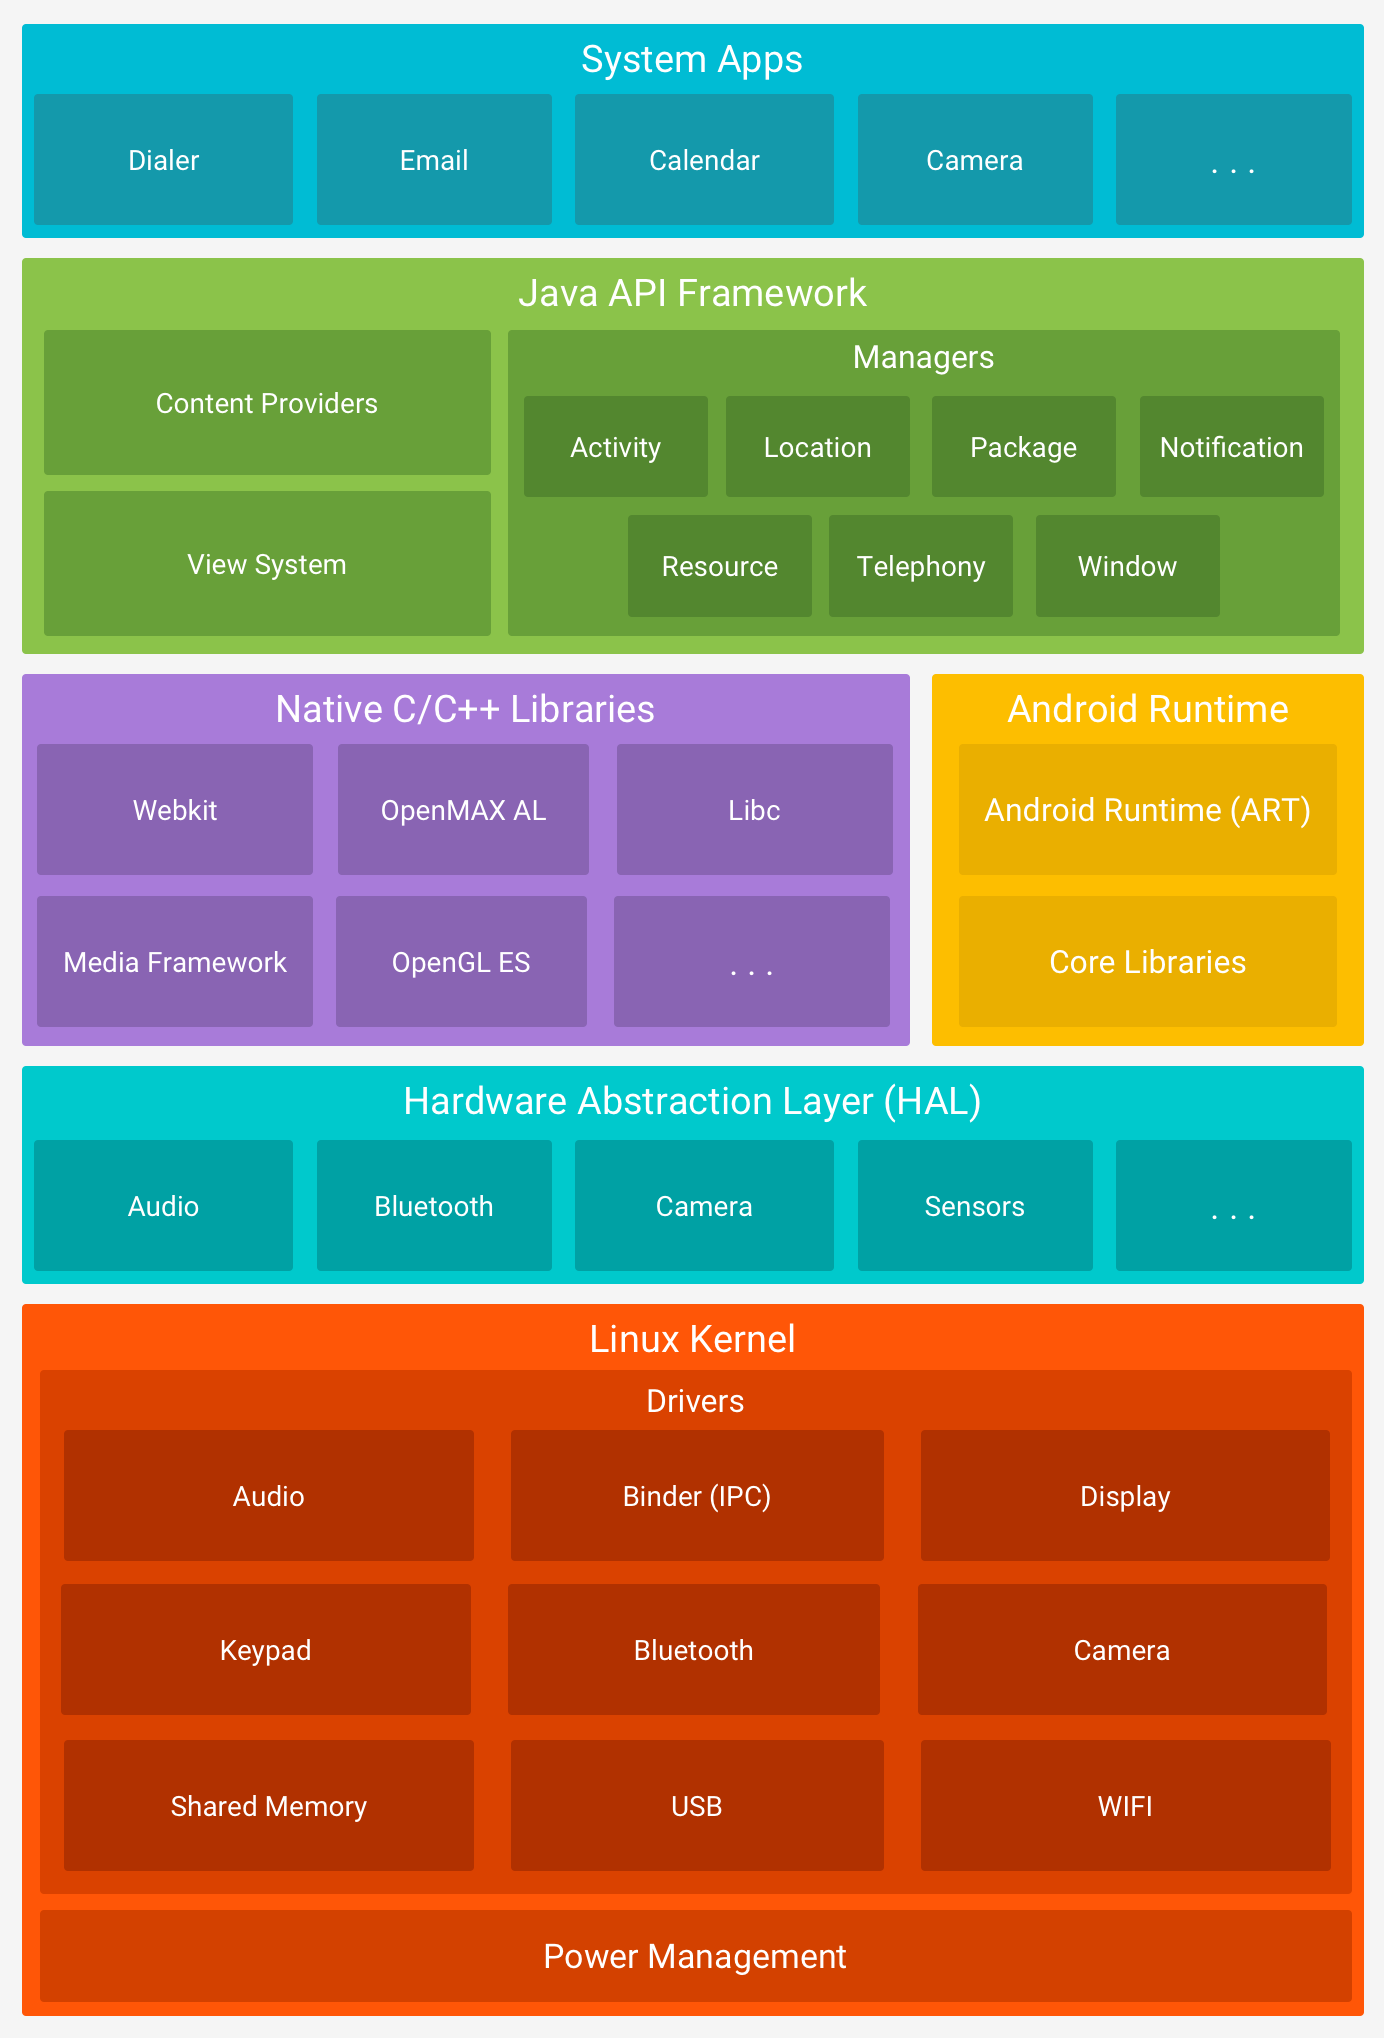
\includegraphics[scale=0.23]{imagenes/android-stack.png}
    \caption{Pila de software de Android}
    \label{fig:android_stack}
\end{figure}

\subsubsection*{Núcleo del sistema operativo: Linux}
\label{section:architecture:kernel}
La base de la plataforma Android es el \textit{kernel} de Linux. Desde el punto de vista de la
seguridad, utilizar a un núcleo tan estudiado a lo largo de los años como pilar de la arquitectura,
ayuda a generar confianza en la misma. Además, le permite a los fabricantes de dispositivos
desarrollar controladores de hardware para un sistema ya conocido.

Una de las principales utilidades de Linux de la que Android toma ventaja es del sistema de permisos
basado en usuarios\footnote{El mismo no debe confundirse con el sistema de permisos implementado por
    Android en una de las capas superiores, que es el que se formaliza y estudia en esta tesina}. Esta
característica permite que cada aplicación sea ejecutada dentro de su propia máquina virtual con un
identificador de usuario único (\texttt{UUID}) asignado a la misma. Luego, por defecto, estos
identificadores se inicializan con permisos de lectura y escritura restringidos, de manera tal que
los recursos de cada aplicación queden debidamente aislados y protegidos de potenciales
\textit{malwares}. Sin embargo, este tipo de defensa, implica la existencia de un mecanismo de
validación de referencia que arbitre las situaciones en las que una aplicación deliberadamente desee
compartir recursos con otra. Este mecanismo es implementado en las capas superiores de la
arquitectura.

Otras características de Linux utilizadas por Android son: la generación de subprocesos, la
administración de memoria de bajo nivel y otras funcionalidades encapsuladas dentro de SELinux
(\textit{\textbf{S}ecurity \textbf{E}nhanced Linux}) como la política de control de acceso
obligatorio (más conocida como \textit{MAC} por sus siglas en inglés) para distinguir entre
aplicaciones del sistema y de terceros.

\subsubsection*{Capa de abstracción de hardware}
Esta capa contiene módulos de software encargados de abstraer los diferentes componentes de
hardware, como la antena de \textit{Bluetooth} o la cámara. Estas abstracciones deben ser
independientes de los \textit{drivers} que se encuentran en el núcleo del sistema, brindando
flexibilidad y transparencia. Cada módulo está autocontenido en una librería, que es cargada
dinámicamente cuando alguna capa superior lo solicita.

\subsubsection*{Entorno de \textit{runtime} y bibliotecas nativas} En esta capa encontramos el
entorno de \textit{runtime} (o ART~\cite{art}, por sus siglas en inglés) utilizado por todas las
aplicaciones del sistema junto con algunas librerías nativas que la plataforma le ofrece a los
desarrolladores.

\subsubsection*{Marco de trabajo/API de la plataforma}
En esta capa se encuentran las interfaces que la plataforma le brinda a los desarrolladores de
aplicaciones para poder acceder a todas las funciones del sistema operativo. Es en esta capa donde
encontramos los servicios que implementan el mecanismo de validación mencionado
\hyperref[section:architecture:kernel]{previamente}.

\subsubsection*{Aplicaciones del sistema y de terceros}
Las aplicaciones representan el escalón final en esta pila de abstracciones, siendo éstas los puntos
de entrada para que cualquier usuario de Android interactúe con las funciones del dispositivo.
Algunas de estas aplicaciones ya vienen preinstaladas en la plataforma (como la de mensajería SMS o
la encargada de brindar la interfaz de configuración del sistema) mientras que otras pueden ser
instaladas a través de la tienda oficial o manualmente.


\section{Conceptos preliminares}
\label{section:preliminary}
El mecanismo que arbitra el acceso a los recursos de las aplicaciones está fuertemente basado en las
interacciones entre las mismas. Por eso, en esta sección introduciremos algunos conceptos que serán
necesarios para un mejor entendimiento del sistema.

\subsection{Componentes de una aplicación}
\label{section:preliminary:components}
Las aplicaciones de Android están conformadas por distintas piezas, que a pesar de ser funcionales
por sí mismas, interactúan entre ellas para otorgar al usuario la funcionalidad esperada. Por
ejemplo, en una aplicación que reproduce música, existirá un componente que se encargará de
presentar la interfaz al usuario mientras que otro, independiente de la interfaz, será el encargado
de reproducir la pista seleccionada. De esta manera, es posible la reproducción de una canción en
segundo~plano\footnote{Una aplicación se considera en segundo plano cuando se está ejecutando a
    pesar de no ser la aplicación que actualmente se está mostrando en la pantalla.}.

Existen cuatro tipos de componentes. Cada uno de ellos representa un punto de entrada por el cual el
sistema o el usuario pueden comunicarse con la aplicación y tiene un ciclo de vida distinto. A
continuación, describiremos brevemente cada uno de ellos.

\paragraph{Actividades:}
Una \textit{actividad} es el punto de entrada de interacción con el usuario, el encargado de ubicar
los elementos en la pantalla. Una aplicación puede tener muchas actividades, cada una de ellas
representando una pantalla distinta. Continuando con el ejemplo de la aplicación para reproducir
música, podríamos pensar que la pantalla del reproductor y la del buscador de canciones son dos
actividades distintas.

\paragraph{Servicios:}
Un \textit{servicio} permite ejecutar procesos en segundo plano. En general, es el encargado de la
ejecución de procesos largos, que de ser interrumpidos podrían afectar el desempeño de la
aplicación. Los servicios son puntos de entrada generales a la aplicación, pueden ser iniciados
tanto por un usuario (a través de una actividad), por otro servicio o por el sistema operativo.

\paragraph{Receptores de anuncios: }
Un \textit{receptor de anuncios} es el componente que se encarga de recibir mensajes del sistema y
de otras aplicaciones, incluso cuando la misma no está en ejecución. Por ejemplo, esta es la forma
en la que el sistema le avisa a todas las aplicaciones que la carga de la batería es baja. Cada
aplicación establece cuáles son los mensajes de su interés, el resto de los mensajes que reciba
simplemente serán ignorados.

\paragraph{Proveedores de contenido:}
El \textit{proveedor de contenido} es el componente encargado de administrar los datos de la
aplicación que se encuentran almacenados en medios persistentes. A través de él, cualquier
aplicación autorizada puede leer o modificar dichos datos. En otras palabras, un proveedor de
contenido actúa como intermediario entre los datos persistidos y las aplicaciones: no solo la dueña
de los datos sino también todas aquellas que hayan sido previamente autorizadas. Cada recurso allí
presente se identifica con un identificador uniforme de recursos (URI).

\subsection{Interacción entre componentes}
Una característica particular de Android es que cualquier aplicación puede iniciar un componente de
otra. Por ejemplo, una aplicación que desee tomar una foto con la cámara del dispositivo, puede
hacerlo \textit{activando} el componente correspondiente de la aplicación provista por el sistema,
en lugar de implementar una nueva actividad que lo haga. Sin embargo, como los procesos de las
aplicaciones ejecutan en procesos aislados y con permisos que limitan el acceso de otras
aplicaciones, el sistema debe actuar como intermediario en la activación de un componente. Para eso,
la aplicación en cuestión debe enviar un \textit{intent} que especifique que lo que desea es iniciar
una actividad en particular. Luego, el sistema será el encargado de activar ese componente.

\subsubsection*{Intents}
Los \textit{intents} son mensajes asíncronos que permiten la comunicación entre componentes y
aplicaciones. Existen tres casos de uso principales: el inicio de una actividad, el inicio de un
servicio y la emisión de un evento, como una indicación de que la batería del dispositivo tiene baja
carga o comenzó a cargarse. Estos mensajes puede ser \textit{explícitos}, en donde el componente de
destino está especificado; o \textit{implícitos}, donde no existe un destinatario específico, pero
el mensaje conlleva la información suficiente para que el sistema encuentre algún componente
apropiado.

\subsubsection*{Filtros de intents}
\label{section:preliminary:intent-filter}
Cuando un intent es implícito, Android busca en los \textit{filtros de intents} de cada aplicación
para verificar cuales de ellas son aptas para recibir ese mensaje. Si un único filtro de intent es
compatible, la aplicación correspondiente será iniciada. Si existe más de uno, el usuario tendrá la
posibilidad de elegir qué aplicación se activará. Los filtros de intent se declaran en el
\textit{manifiesto} de la aplicación y por lo tanto, son estáticos.

\subsection{Manifiesto de la aplicación}
\label{section:preliminary:manifest}
El archivo de manifiesto de una aplicación es un documento \texttt{xml} que contiene información
estática sobre la misma. Su tarea principal es declarar cuáles son los componentes que corresponden
a la aplicación, para que de esta forma, el sistema pueda reconocerlos como tales. Algunas otras
declaraciones que se encuentran en el manifiesto son:
\begin{enumerate}
    \item El nombre del paquete de la aplicación.
    \item Los filtros de intents \hyperref[section:preliminary:intent-filter]{previamente
              mencionados}.
    \item Los aspectos de hardware y software que la aplicación utilizará, como una cámara o los
          servicios de Bluetooth.
    \item Los permisos de usuario que requiere la aplicación
\end{enumerate}

\section{Mecanismo básico de protección: permisos}
\label{section:android:permissions}
Como ya mencionamos en la sección \ref{section:architecture:kernel}, existe en Android un mecanismo
encargado de arbitrar el acceso a la información sensible de las aplicaciones y a algunos recursos
del sistema. Este mecanismo, al que a lo largo de este trabajo llamaremos \textit{sistema de
    permisos}, cumple un rol fundamental en el modelo de seguridad de Android. Este sistema fue el que
se ha estudiado en profunidad y formalizado en esta tesina.

A grandes rasgos, para que una aplicación pueda acceder a un recurso sensible, tanto del sistema
como de otra aplicación, debe haber obtenido previamente los permisos necesarios. De ser así, la
operación es realizada con éxito. Caso contrario, la aplicación debe pedirle al sistema operativo
que le otorgue el o los permisos en cuestión. Finalmente, el sistema operativo, dependiendo del
\textit{nivel de protección} de dicho permiso, puede delegar la decisión al usuario a través de
una ventana emergente. Análogamente, si un desarrollador desea proteger un recurso de su aplicación,
puede definir un nuevo permiso y establecer que el recurso solo puede ser compartido con aquellas
otras aplicaciones que cuenten con el mismo. De esta forma, nos encontramos con una primer
clasificación entre permisos: aquellos definidos por las aplicaciones para mantener sus datos
protegidos; y los definidos por el sistema, que se necesitan para ganar acceso a los recursos del
dispositivo que pueden comprometer la privacidad del usuario (como la cámara o la lista de
contactos).

Cada permiso tiene un nombre único y cuenta un nivel de protección. El nivel de protección determina
de qué forma procederá el sistema operativo cuando un permiso es solicitado. Existen tres niveles:

\begin{enumerate}
    \item \textbf{Normal:} Estos permisos pueden ser otorgados automáticamente por el sistema ya que
          se utilizan para información o recursos que tienen un riesgo muy bajo de comprometer la
          seguridad.
    \item \textbf{Peligrosos:} Los permisos de este nivel protegen recursos mucho más sensibles y
          requieren la aprobación explícita del usuario.
    \item \textbf{De misma firma:} Un permiso de este tipo se otorga solamente si la aplicación que
          lo está solicitando y la aplicación que lo declara están firmadas con el mismo
          certificado.
\end{enumerate}

A partir de la versión \texttt{6} de Android, todos los permisos peligrosos se otorgan en tiempo de
ejecución mientras que los correspondientes a los otros niveles se conceden en el momento en el que
la aplicación se instala.

Los permisos que están asociados a una misma característica de la aplicación o dispositivo,
suelen estar agrupados. Por ejemplo, tanto el permiso necesario para leer los mensajes de texto,
como el que autoriza el envío de los mismos, pertenecen a un mismo \textit{grupo de permisos}
llamado \texttt{SMS}. El principal objetivo de agrupar permisos es evitar abrumar al usuario con
preguntas sobre la concesión de los mismos. De esta forma, si una aplicación requiere un permiso
peligroso que está agrupado, el sistema le pedirá que autorice a todo el grupo. En la sección
\ref{subsection:recent-changes:grouped-permissions}, estudiaremos más en detalle qué significa
autorizar a un grupo, dependiendo de la versión de Android que se analice.

\subsection*{Delegación de permisos}
Existen dos mecanismos mediante los cuales una aplicación puede delegar sus propios permisos a otra.
El primero consiste en dejar un \texttt{Intent} pendiente, para que otra aplicación pueda tomarlo y
ejecutarlo con los permisos y la identidad de quien lo creó. El segundo método, en cambio, consiste
en que una aplicación que cuenta con permisos de escritura/lectura sobre un proveedor de contenido
puede delegar \textit{temporalmente} esos permisos a otra aplicación. Los permisos delegados serán
revocados una vez que la actividad o servicio que los recibió haya terminado su ejecución.

\section{Cambios recientes}
\label{section:recent-changes}
En esta sección analizamos informal y brevemente los cambios que fueron introducidos entre Android
Nougat (7) y Andrid 10 que tuvieron un impacto significativo en el sistema de permisos.

\subsection{Sistema de archivos}
\label{subsection:recent-changes:filesystem}
Con intención de aumentar la seguridad de las aplicaciones, el directorio privado de todas aquellas
orientadas\footnote{
    Las aplicaciones pueden estar orientadas a distintas versiones del sistema. Android utiliza esta
    configuración para determinar la compatibilidad de ciertos comportamientos nuevos.
} a una versión posterior a Android 7 tienen permisos restringidos. Solamente la aplicación dueña
puede leer, escribir y ejecutar. Esta configuración evita la fuga de metadatos de los archivos
privados, como el tamaño o su existencia. De esta forma, las aplicaciones ya no pueden otorgar
permisos de lectura/escritura a otras para compartir sus archivos, sino que deben hacerlo otorgando
permisos temporales mediante un proveedor de contenido.

El modelo de Android del cual partimos en esta tesina, ya contemplaba el otorgamiento temporal de
permisos de lectua/escritura. Además, decidimos \textbf{no} modelar el sistema de archivos de
Android en este trabajo, dado que nuestro interés se centra en estudiar propiedades más generales
relacionadas a los permisos y creemos que el modelado de un sistema de archivos require un gran
esfuerzo que no aporta hacia donde queremos llegar. Por lo tanto, no se introdujeron cambios en el
modelo con respecto a esta nueva característica.

\subsection{Comportamiento de permisos agrupados}
\label{subsection:recent-changes:grouped-permissions}
En versiones previas a Android 8, si una aplicación solicitaba un permiso agrupado y el permiso era
otorgado, el sistema también otorgaba el resto de los permisos del mismo grupo que estuvieran
declarados en el manifiesto. Este comportamiento se consideraba incorrecto ya que violaba el
principio de mínimo privilegio en la plataforma. A partir de la octava versión de Android,
este comportamiento ha cambiado. Cuando una aplicación pide un permiso agrupado y lo consigue, solo
obtiene el permiso que fue explícitamente solicitado. Sin embargo, si posteriormente desea conseguir
otro permiso perteneciente al mismo grupo, el sistema tiene autorización para otorgarlo
automáticamente. En otras palabras, cuando una aplicación solicita un permiso \textbf{peligroso}
agrupado por primera vez, el usuario será quien determine si ese permiso es otorgado o no; pero las
solicitudes posteriores de permisos del mismo grupo serán automáticamente aceptadas por el sistema.

Desde un punto de vista conceptual, este cambio es muy favorable en pos de respetar el principio de
mínimo privilegio. Sin embargo, cabe preguntarse por qué simplemente no se delega al usuario la
autorización de cada uno de los permisos peligrosos que una aplicación solicita, que desde el punto
de vista de dicho principio, es una implementación óptima. La respuesta está en la negociación que
los autores de la plataforma deben mediar entre políticas muy estrictas de seguridad y una buena
experiencia de usuario (invadir al usuario de advertencias y solicitudes no es algo favorable en ese
sentido).

A pesar de lo mencionado en el párrafo anterior, si miramos los cambios introducidos en esta versión
desde un lugar de seguridad más concreto, seguimos encontrando situaciones peligrosas como la que
describimos a continuación.

% Cabe preguntarse por qué simplemente no se El \textit{quid} de la cuestión detrás de garantizar
% automáticamente las solicitudes subsecuentes de permisos del mismo grupo es reducir la cantidad de
% alertas que se muestran en pantalla para una mejor experiencia de usuario. 
\subsubsection{Permisos peligrosos y normales en el mismo grupo}
De acuerdo a la documentación de Android, ``cualquier permiso puede pertenecer a un grupo de
permisos sin importar el nivel del protección del mismo''~\cite{android-permissions}. Sin embargo, en
ningún lugar se especifica si permisos de distintos niveles de protección (en particular, uno de
nivel normal y otro peligroso) pueden compartir el mismo grupo ni, en caso de que sea posible, cómo
debería el sistema manejar el otorgamiento automático de permisos. De aquí se desprenden algunas
preguntas interesantes:
\begin{enumerate}
    \item Dado que los permisos normales se otorgan en tiempo de instalación y sin explícita
          aprobación del usuario, ¿habilita esto el posterior otorgamiento automático de los
          permisos peligrosos del mismo grupo? ¿Se informa de esta decisión al usuario?
    \item De no ser así, ¿cómo se encarga el sistema de manejar esta situación?
\end{enumerate}
En esta tesina formalizamos el peor de los escenarios, en donde un permiso normal puede habilitar el
otorgamiento automático de un permiso peligroso sin que el usuario se entere. Este escenario sigue
siendo válido dada la especificación informal de la plataforma. Analizaremos esto formalmente en la
sección siguiente.


\subsection{Cambios en pos de la privacidad del usuario}
Tanto en Android 9 como en Android 10 se introdujeron varios cambios que apuntan a mejorar la
privacidad de los usuarios. Entre ellos, destacamos:
\begin{enumerate}
    \item Acceso limitado a los sensores del dispositivo cuando las aplicaciones se ejecutan en
          segundo plano. Por ejemplo, las aplicaciones ya no pueden acceder ni al micrófono ni a la
          cámara sin notificar al usuario.
    \item Acceso restringido al registro de llamadas y a números telefónicos.
    \item Acceso restringido a la información obtenida de un análisis de Wi-Fi.
    \item Se agregó un permiso (peligroso) para acceder a la ubicación en segundo plano.
    \item Se agregaron restricciones sobre cuándo un servicio puede empezar una actividad. De esta
          manera, se busca que el usuario tenga más control sobre lo que ve en su pantalla.
\end{enumerate}

Sin embargo, todos estos cambios son específicos a la implementación y no tienen impacto en una
representación abstracta como la nuestra.

\subsection{Chequeo de permisos en aplicaciones \textit{legacy}}
\label{subsection:recent-changes:legacy-apps}

A partir de Android 10, cuando una aplicación orientada a una versión previa a Android 6 es
ejecutada por primera vez, el usuario será alertado. Además, dado que en las versiones más viejas de
la plataforma los permisos peligrosos se otorgaban al momento de la instalación, el usuario ahora
tendrá la posibilidad de revisar los mismos antes de que la aplicación se ejecute. Este cambio
fue formalizado e incluido en nuestro modelo.



\chapter{Formalización del sistema de permisos}
\label{chapter:formalization}

En este capítulo describiremos la extensión que realizamos sobre una formalización
previa\cite{luna-cleiej} del sistema de permisos de la plataforma para modelar los nuevos
comportamientos que se introdujeron con las versiones 7, 8, 9 y 10 del sistema operativo. También
presentaremos las propiedades más importantes que extrajimos del modelo, focalizándonos en aquellas
nuevas o en las que se han visto considerablemente afectadas en las nuevas versiones.


\section{Lenguaje formal utilizado}
\label{section:formalization:formal-language}
La especificación del sistema se realizó dentro del framework de trabajo Coq~\cite{coq}. Coq es un
asistente de pruebas interactivo, que permite el desarrollo de programas consistentes con su especificación.
Para lograrlo, provee tres aspectos fundamentales:
\begin{enumerate}
    \item Un lenguaje de especificación que permite escribir expresiones lógicas de alto orden, algoritmos y teoremas;
    \item Un asistente de pruebas que permite desarrollar pruebas matemáticas verificadas;
    \item Una herramienta de extracción de programas, que permite sintetizar programas en lenguajes
          como OCaml~\cite{ocaml} o Haskell~\cite{haskell} a partir de las especificaciones formales escritas
          previamente. Los programas construidos de esta manera suelen llamarse \textit{programas
              certificados}.
\end{enumerate}

El lenguaje lógico subyacente usado por Coq es el Cálculo de Construcciones Inductivas~\cite{cic}
(también conocido como CIC, por sus siglas en inglés).

\section{Notación}
En las siguientes secciones  utilizaremos la misma notación de los trabajos
previos~\cite{luna-cleiej,betarte-2017,betarte-2016}. La misma es similar a la sintaxis de Haskell.

\subsection{Estructuras de datos y tipos generales}
TODO: COMPLETAR ESTA SECCIÓN

Los diccionarios (más conocidos como \textit{records} por su nombre en inglés) tendrán la forma $\{
    l_1: T_1, ..., l_n: T_n \}$ y notaremos el acceso a cada uno de sus elementos como $r.l_n$. También
usaremos $\{ T \}$ para definir el tipo del conjunto que contiene elementos de tipo $T$.

Definir tipos inductivos blablabla

Para denotar el tipo de las funciones utilizaremos el símbolo $ \rightarrow$. Por ejemplo, una función
$f$ que toma un argumento de tipo $A$ y uno de tipo $B$ y devuelve un valor de tipo $C$, se notará
como $F: A \rightarrow B \rightarrow C$. Usaremos siempre la notación currificada.

\subsection{Tipos básicos de Coq}
A continuación detallaremos algunos de los tipos básicos de Coq más utilizados en esta tesina.
\subsubsection*{Tipo \textit{option}}
\begin{flalign*}
    Inductive\ option\ T\ &:= &&\\
    &|\ Some\ :\ T \rightarrow\ option\ T&&\\
    &|\ None\ :\ option\ T &&
\end{flalign*}


El tipo \texttt{option}, análogo a la mónada \texttt{Maybe} de Haskell\cite{maybe-haskell}, sirve para
representar la posible ausencia de valores. Dado que en Coq no es posible definir funciones
parciales, utilizaremos este tipo para totalizar a las mismas. De esta manera, una función parcial $g$
de $A$ en $B$, será definida como $g:\ A\ \rightarrow\ option\ B$.

\subsubsection*{Tipo \textit{list}}
\begin{flalign*}
    Inductive\ list\ T\ &:= &&\\
    &|\ \texttt{(::)}\ :\ T \rightarrow\ list\ T\ \rightarrow\ list\ T\ &&\\
    &|\ nil\ :\ list\ T &&
\end{flalign*}

El tipo utilizado para denotar una lista de elementos. Está definido de manera inductiva, siendo
\texttt{::} un operador de punto fijo.

\subsubsection*{Tipo \textit{nat}}
Utilizado para denotar a los números naturales.

\subsubsection*{Tipo \textit{Prop}}

Este tipo representa uno de los dos "universos" donde viven las proposiciones lógicas en Coq. El tipo
$Prop$ es impredicativo y por lo tanto, una proposición de este tipo no contiene valor
computacional\cite{proof-irrelevance} y puede ser descartada a la hora de extraer un programa.
Utilizaremos este tipo para escribir teoremas que nos permitan razonar sobre el modelo. El otro
universo que contiene proposiciones lógicas se llama $Set$ y las proposiciones de este tipo sí tienen
valor computacional y deben ser preservadas en los programas extraídos.


\section{Estado del sistema}
\label{section:formalization:state}

\subsection{Formalización de los componentes básicos}
En esta sección presentaremos las estructuras de datos utilizadas para formalizar los distintos
componentes presentados en la sección \ref{section:preliminary}. El orden en el que introduciremos
dichas abstracciones será incremental con respecto a la complejidad de las mismas y por lo tanto,
diferirá del orden en el que los componentes fueron presentados anteriormente.

\subsubsection*{Tipos atómicos}
En la tabla \ref{table:atomic_types} se enumeran las estructuras de datos atómicas. Entendemos por
estructura de dato atómica a aquellas que representan tipos básicos o bien, a aquellas cuya definición
queda sujeta a cuestiones de implementación. En el asistente de pruebas Coq, estas estructuras fueron
definidas como parámetros de tipo $Set$.


\begin{table}[thb!]
    \centering
    \begin{tabularx}{\linewidth}{|l X|}
        \hline
        \textbf{Nombre del tipo} & \textbf{Descripción}                                                                                                  \\
        \hline
        $idApp$                  & Identificadores/nombres de las aplicaciones.                                                                          \\
        \hline
        $idPerm$                 & Identificadores/nombres de los permisos.                                                                              \\
        \hline
        $idGrp$                  & Identificadores/nombres de los grupos de permisos.                                                                    \\
        \hline
        $idCmp$                  & Identificadores/nombres de los componentes de una aplicación.                                                         \\
        \hline
        $iCmp$                   & Identificadores/nombres de las instancias en ejecución de los componentes de una aplicación.                          \\
        \hline
        $uri$                    & Identificadores de los recursos guardados en los proveedores de contenido.                                            \\
        \hline
        $res$                    & Recursos definidos por los proveedores de contenido.                                                                  \\
        \hline
        $mimeType$               & Parámetro utilizado para representar los distintos tipos de
        MIME\cite{mime-types}. Este tipo de datos es utilizado por los $intents$ y los filtros de
        $intents$ para saber cómo decodificar la información allí almacenada.                                                                            \\
        \hline
        $Category$               & Categoría a la que puede pertenecer un $intent$.                                                                      \\
        \hline
        $Cert$                   & Certificados con los que se firman las aplicaciones.                                                                  \\
        \hline
        $Extra$                  & Abstracción usada para representar el campo de información "extra" que puede enviarse a través de los $intents$.      \\
        \hline
        $Flag$                   & Banderas que pueden ser activadas por el emisor de un $intent$ para indicar cómo debe leerse/manejarse ese mensaje.   \\
        \hline
        $SACall$                 & Llamadas a la API de Android que interfieren con el modelo de seguridad (por ejemplo, para tener acceso a internet).  \\
        \hline
        $Val$                    & Tipo genérico para representar valores. Usado para representar los valores de los recursos ($res$) de una aplicación. \\
        \hline
        $vulnerableSdk$          & SDK a partir del cual las aplicaciones empiezan a considerarse como
        $legacy$ y requieren una verificación del usuario antes de ser ejecutadas por primera vez.                                                       \\
        \hline
    \end{tabularx}
    \caption{Tipos atómicos}
    \label{table:atomic_types}
\end{table}


\subsubsection*{Permisos}
Los permisos descriptos en la sección \ref{section:android:permissions} fueron formalizados como un
registro de tres campos: el nombre o identificador del permiso en cuestión, el nombre o identificador del
grupo al que pertenece el permiso (en caso de que no pertenezca a ningún, lo representaremos mediante el
valor \textit{None}) y el nivel de protección del mismo. Formalmente,

\begin{align*}
    Perm\ :=\ \{ idP: idPerm;\ maybeGrp: option\ idGrp;\ pl: permLevel \}
\end{align*}

El tipo de datos \textit{permLevel} es un tipo de datos enumerado cuyos valores posibles son:
\textit{normal}, \textit{dangerous} y \textit{signature}. Cada uno de estos valores representa uno de los
niveles de protección descriptos en la sección \ref{section:android:permissions}.

\subsubsection*{Intents}
De manera análoga a los permisos (y a la mayoría de los componentes que mencionaremos), también
utilizamos registros para formalizar a los \textit{intents}. En este caso, los registros poseen una mayor
cantidad de campos, algunos de ellos representados con estructuras complejas como un nuevo registro. Los
nueve campos que definen a un \textit{intent} son:

\begin{itemize}
    \item \textit{idI}, el nombre o identificador del intent,
    \item \textit{cmpName}, en caso de que el intent esté dirigido a un componente en particular, el
    identificador del mismo
    \item \textit{intType}, define el caso de uso del intent. Puede ser: iniciar una actividad, iniciar
    un servicio o transmitir un evento por \textit{broadcast} a cualquier aplicación interesada
	\item \textit{action}, la acción que ejecutará el intent. Por ejemplo, el valor \texttt{ACTION\_VIEW}
	en este campo junto con el \texttt{URI} de un contacto, resultará en el sistema mostrando la
	información de dicho contacto
    \item \textit{data}, contiene la información necesaria para identificar los datos que son necesarios
    para ejecutar la acción en cuestión
    \item \textit{category}, contiene información adicional sobre la acción a ejecutar
    \item \textit{extra}, contiene información adicional de cualquier tipo
    \item \textit{flags}, banderas que contienen información sobre cómo manejar el \textit{intent}
    \item\textit{brperm}, en caso de que el componente que recibe el intent necesite un permiso para
    ejecutarlo, el mismo deberá estar listado aquí
\end{itemize}


Formalmente, un \textit{intent} está definido con la siguiente estructura:

\begin{align*}
    Intent\ &:=\ \{ \\
        &idI: idInt; \\
        &cmpName: option\ idCmp; \\
        &intType: intentType \\
        &action: option\ intentAction \\
        &data: Data \\
        &category: list\ Category \\
        &extra: option\ Extra \\
        &flags: option\ Flag \\
        &brperm: option\ Perm \\
    \}
\end{align*}

La estructura $Data$ está definida a su vez como un record que contiene un URI al recurso que obtendrá
quien reciba el intent, el tipo de dato al que se intentará acceder y, opcionalmente, el tipo de dato en
formato MIME.

\begin{align*}
    Data\ :=\ \{ path: option\ uri;\ type: dataType;\ mime: option mimeType \}
\end{align*}

La estructura $dataType$ es una enumeración que contiene los siguientes valores: $content$, $file$ y
$other$.


\subsection{Definición de estado}
Nuestra formalización del sistema de permisos de Android puede pensarse como una máquina de estado
abstracta [CITA?]. En este modelo, los estados del sistema están conformados por dos componentes: uno
que almacena la información dinámica del sistema, como las aplicaciones instaladas y los permisos otorgados
a las mismas; y otro que contiene información estática como el manifiesto de cada aplicación. Formalmente:

\begin{align*}
    System\ :=\ \{ state: State;\ environment: Environment \}
\end{align*}


El componente $State$ está conformado por los siguientes elementos:

\begin{itemize}
    \item Una lista con los identificadores de las aplicaciones instaladas,
    \item Una lista  información de las aplicaciones \textit{legacy} que ya han sido verificadas por
          el usuario. Es un subconjunto de las aplicaciones inst.
    \item Un mapeo entre las aplicaciones instaladas y los permisos otorgados a cada una de ellas.
    \item Un mapeo entre las aplicaciones instaladas y los grupos de permisos para los cuales el
          usuario ha permitido el otorgamiento automático de permisos.
    \item Un mapeo entre los componentes que define una aplicación y las instancias en ejecución de
          ellos.
    \item Un mapeo entre los recursos de un proveedor de contenidos para una aplicación y los permisos
          permantentes otorgados sobre el mismo.
    \item Un mapeo entre los recursos de un proveedor de contenidos para una aplicación y los permisos
          temporales otorgados sobre el mismo.
    \item Un mapeo indicando el valor de cada uno de los recursos de una aplicación.
    \item Una lista de los intents que han sido enviados, junto con su emisor.
\end{itemize}

Por otro lado, el componente $Environment$ contiene la siguiente información:

\begin{itemize}
    \item Un mapeo que asocia a cada aplicación con su archivo de manifiesto
    \item Un mapeo que asocia a cada aplicación con el certificado que se utilizó para firmarla
    \item Un mapeo que asocia a las aplicaciones con los permisos definidos por ellas
    \item Una lista de las aplicaciones pre-instaladas del sistema
\end{itemize}

A continuación daremos la definición formal de ambos componentes. El orden en el que se definen los
campos de cada componente es el mismo que el de las numeraciones previas.
\begin{flalign*}
    State\ &:=\ \{ &&\\
    &apps:\ list\ idApp; \\
    &alreadyVerified:\ list\ idApp; \\
    &grantedPermGroups:\ mapping\ idApp\ (list\ idGrp); \\
    &perms:\ mapping\ idApp\ (list\ Perm); \\
    &running:\ mapping\ iCmp\ Cmp; \\
    &delPPerms:\ mapping\ (idApp\ *\ CProvider\ *\ uri)\ PType; \\
    &delTPerms:\ mapping\ (iCmp\ *\ CProvider\ *\ uri)\ PType; \\
    &resCont:\ mapping\ (idApp\ *\ res)\ Val; \\
    &sentIntents:\ list\ (iCmp*Intent) \\
    \}
\end{flalign*}

\begin{flalign*}
    Environment\ &:=\ \{ &&\\
    &manifest:\ mapping\ idApp\ Manifest; \\
    &cert:\ mapping\ idApp\ Cert; \\
    &defPerms:\ mapping\ idApp\ (list\ Perm); \\
    &systemImage:\ list\ SysImgApp; \\
    \}
\end{flalign*}

De aquí en adelante, al hablar del estado del sistema, nos estaremos refiriendo al componente
$System$. En caso de que querramos referirnos a alguno de sus subcomponentes seremos explícitos con su
nombre en inglés.

\subsubsection{Estados válidos del sistema}
No todos los elementos que habitan el conjunto definido anteriormente son relevantes al sistema que
queremos estudiar. Por ejemplo, no queremos trabajar sobre un estado en el que una aplicación
pre-instalada del sistema y una aplicación instalada por el usuario puedan tener el mismo
identificador.

Inicialmente, a la hora de definir los componentes, fue necesario pensar qué condiciones debían
cumplir estos estados para representar estados de Android que tengan sentido. En consecuencia,
definimos una noción de \textbf{estado válido} para restringir el universo de estados a aquellos que
cumplen ciertas condiciones que nos garantizarán que nuestros estados del modelo tienen sentido al
compararlos con estados reales del sistema. Vale aclarar, que nuestra definición de estado válido no
es completa y que, de alguna manera, está focalizada en las propiedades que probaremos luego.

Se definió formalmente un predicado $valid\_state$ que se satisface cuandos se cumplen las siguientes
condiciones:

\begin{itemize}
    \item Todos los componentes, ya sea que pertenezcan a una aplicación instalada por el usuario o a
          una aplicación pre-instalada en el sistema tienen identificadores diferentes.
    \item Ningún componente pertenece a más de una aplicación.
    \item Ningún componente en ejecución es una instancia de un proveedor de contenido (los mismos no se \textit{ejecutan}).
    \item Todo permiso temporalmente otorgado ha sido otorgado a un componente en ejecución y es sobre
          un recurso de un proveedor de contenido existente.
    \item Todo componente en ejecución pertenece a una aplicación instalada en el sistema.
    \item Toda aplicación que establece un valor a un recurso está instalada en el sistema.
    \item El dominio de las funciones parciales que definen el $manifest$, $cert$ y $defPerms$ es el
          conjunto de todas las aplicaciones instaladas por el usuario.
    \item El dominio de las funciones parciales que definen $grantedPermGroups$ y $perm$ es el
          conjunto de todas las aplicaciones del sistema, tanto instaladas por el usuario como
          pre-instaladas.
    \item Todas las aplicaciones del sistema tienen identificadores diferentes.
    \item Todos los permisos definidos por las aplicaciones tienen identificadores diferentes.
    \item Todos los permisos otorgados existen en el sistema.
    \item Todos los intents que han sido enviados tienen identificadores diferentes.
\end{itemize}

\section{Acciones}
Modelamos las operaciones de Android que nos interesan estudiar como un conjunto de acciones
(definidas a través del tipo \texttt{Action}), donde cada una de ellas determina la manera en la que
nuestro sistema puede transicionar.  La tabla~\ref{table:actions} resume todas las acciones
disponibles.

La semántica de las mismas está dada en términos de pre-condición y post-condición. Para ello,
definimos los predicados $Pre$ y $Post$ de manera tal que para que una acción $a$ pueda transicionar
el sistema desde un estado $s$ hacia otro estado $s'$, deberán cumplirse $Pre\ s\ a$ y $Post\ s\ s'\
    a$. Notaremos la transición de un estado a otro de la siguiente manera: $s\ \step{a}\ s'$.

A continuación y a modo de ejemplo, describiremos informalmente las acciones que han sido introducidas
o modificadas con las últimas actualizaciones del sistema.

\subsubsection{Semántica de \texttt{grant}}

Esta operación es la encargada de otorgar un permiso $p$ a una aplicación $a$. La misma ya estaba
presente en la formalización de la que se partió en esta tesina. Sin embargo, su semántica ha sido
modificada a raíz de las actualizaciones de la plataforma mencionadas en la sección
\ref{subsection:recent-changes:grouped-permissions}. En particular, ahora el sistema podrá
transicionar con esta operación solo si  el permiso $p$ no pertenece a un grupo o, en caso de que
pertenezca, es el primero del grupo en ser otorgado a la aplicación. El resto de las precondiciones
necesarias para transicionar se mantuvieron: el permiso $p$ debe existir (es decir, debe estar
definido o bien por el sistema o por alguna aplicación), debe estar declarado como usado en el
manifiesto de la aplicación $a$, debe ser un permiso peligroso y no debe haber sido otorgado a la
aplicación previamente.

Si la precondición se cumple, el sistema transicionará hacia un estado en dónde el permiso se agrega a
los permisos otorgados a la aplicación, es decir, se agrega $p$ al conjunto $perms\ a$; y en caso de
corresponder, ocurre lo análogo con el grupo de $p$ y $grantedPermGroups\ a$. El resto de los
componentes del sistema no se verán modificados.

\subsubsection{Semántica de \texttt{grantAuto}}

Para modelar en su totalidad a los cambios mencionados en la sección
\ref{subsection:recent-changes:grouped-permissions}, además de los cambios en la semántica a la
operación \texttt{grant}, se introdujo una nueva acción \texttt{grantAuto}. Esta última difiere de la
primera en que el sistema solo podrá transicionar con ella si el permiso que se intenta otorgar
pertenece a un grupo que el usuario ya ha autorizado. En caso de que esto se cumpla, el modelo mutará
hacia un estado en donde la aplicación en cuestión obtuvo el permiso solicitado.

\subsubsection{Semántica de \texttt{revoke} y \texttt{revokePermGroup}}

De manera similar a lo ocurrido con \texttt{grant} y \texttt{grantAuto}, la semántica de las
operaciones  \texttt{revoke} y \texttt{revokeGroup} también se modificaron con los cambios de las
últimas versiones. Decidimos modelar estas operaciones de manera tal que se mantenga una relación con
la experiencia de usuario al revocar permsisos. De esta manera, la operación \texttt{revoke} es la
encargada de revocar permisos individuales \textbf{no} agrupados mientras que \texttt{revokePermGroup}
quita todos los permisos pertenecientes al grupo deseado. Nuestro modelo no permite revocar permisos
que pertenezcan a un grupo de manera individual.

Si el sistema transiciona con \texttt{revoke}, entonces dado un permiso $p$ y una aplicación $a$,
obtendremos un estado en donde la aplicación $a$ ya no tendrá acceso a los recursos protegidos por
$p$. Análogamente, dado un permiso $g$ y una aplicación $a'$, al transicionar con
\texttt{revokePermGroup}, la aplicación $a$ ya no tendrá ningún permiso perteneciente al grupo $g$.
Además, el sistema ya no estará autorizado a otorgar a la aplicación $a$ permisos del grupo $g$ de
manera automática.


\subsubsection{Semántica de \texttt{verifyOldApp}}

Esta operación se agregó al modelo para razonar sobre el nuevo el comportamiento mencionado en la
sección~\ref{subsection:recent-changes:legacy-apps}. Dada una aplicación $a$, para poder transicionar
el sistema utilizando la operación $verifyOldApp\ a$, deben cumplirse las siguientes condiciones: $a$
debe ser una aplicación instalada en el sistema, aún no debe haber sido ejecutada y debe estar
orientada a una versión previa a la sexta versión de Android.

En la implementación real de la plataforma, al momento de verificar una aplicación vieja se muestra al
usuario un menú con los permisos otorgados a la misma en el momento en que fue instalada, junto
con la posibilidad de elegir cuales de ellos se desea mantener y cuales revocar. Nuestra operación
$verifyOldApp\ a$ simplemente transiciona hacia un estado en donde a la aplicación $a$ se le han
revocado todos sus permisos y se ha marcado como verificada. Para modelar la acción en la que el
usuario selecciona los permisos que desea mantener mediante la interfaz ofrecida por Android,
deberemos dar una sucesión de acciones,  donde primero se verifica la aplicación y luego se otorgan
los permisos que se eligió mantener.

\subsubsection{Semántica de \texttt{receiveIntent}}

A raíz del cambio mencionado previamente y en la sección~\ref{subsection:recent-changes:legacy-apps},
agregamos una nueva condición que deberá cumplirse para que una aplicación pueda recibir un
\textit{intent}: para que una aplicación $a$ pueda recibir el intent $i$, entonces la misma no debe
ser una aplicación \textit{legacy} o, en caso de serlo, debe haber sido previamente verificada por el
usuario.

\begin{table}
    \label{table:actions}
    \vspace{0.2cm}
    \begin{tabularx}{\linewidth}{|l X|}
        \hline
        \textbf{Acción}   & \textbf{Descripción}                                                                                                                                               \\
        \hline
        $\mathtt{install}~app~m~c~res$     & Instala la aplicación con identificador $app$, cuyo manifiesto es $m$, su certificado es $c$ y la lista de recursos es $res$.                                                                                        \\
        \hline
        $\mathtt{uninstall}~app$           & Desinstala la aplicación con identificador $app$.                                                                                                                                                                    \\
        \hline
        $\mathtt{read}~ic~cp~u$            & El componente en ejecución $ic$ lee el recurso correspondiente al identificador URI $u$ del proveedor de contenido $cp$.                                                                                             \\
        \hline
        $\mathtt{write}~ic~cp~u~val$       & El componente en ejecución $ic$ escribe el valor $val$ en el recurso correspondiente al identificador $u$ del proveedor de contenido $cp$.                                                                           \\
        \hline
        $\mathtt{startActivity}~i~ic$      & El componente en ejecución $ic$ solicita comenzar la actividad especificada por el intent $i$.                                                                                                                       \\
        \hline
        $\mathtt{startActivityRes}~i~n~ic$ & El componente en ejecución $ic$ solicita comenzar la actividad especificada por el intent $i$ y espera como respuesta un token $n$.                                                                                  \\
        \hline
        $\mathtt{startService}~i~ic$       & El componente en ejecución $ic$ solicita comenzar el servicio especificado por el intent $i$.                                                                                                                        \\
        \hline
        $\mathtt{sendBroadcast}~i~ic~p$    & El componente en ejecución $ic$ envía el intent $i$ en modo \textit{broadcast}, especificando que solo los componentes que posean el permiso $p$ pueden recibirlo.                                                   \\
        \hline
        $\mathtt{sendOrdBroadcast}~i~ic~p$ & El componente en ejecución $ic$ envía el intent $i$ en modo \textit{broadcast} ordenado,  especificando que solo los componentes que posean el permiso $p$ pueden recibirlo.                                         \\
        \hline
        $\mathtt{sendSBroadcast}~i~ic$     & El componente en ejecución $ic$ envía el intent $i$ en modo \textit{sticky broadcast}.                                                                                                                               \\
        \hline
        $\mathtt{resolveIntent}~i~app$     & La aplicación $app$ vuelve al intent $i$ explícito.                                                                                                                                                                  \\
        \hline
        $\mathtt{stop}~ic$                 & El componente en ejecución $ic$ termina su ejecución.                                                                                                                                                                \\
        \hline
        $\mathtt{grantP}~ic~cp~app~u~op$   & El componente en ejecución $ic$ delega permisos permantentes a la aplicación $app$. Esta delegación autoriza a $app$ a realizar la operación $op$ en el recurso asignado al URI $u$ del proveedor de contenido $cp$. \\
        \hline
        $\mathtt{revokeDel}~ic~cp~u~op$    & El componente en ejecución $ic$ revoca los permisos otorgados al recurso $u$ del proveedor de contenidos $cp$ para realizar la operación $op$.                                                                       \\
        \hline
        $\mathtt{call}~ic~sac$             & El componente en ejecución $ic$ realiza el llamado a una función del sistema denominada $sac$.                                                                                                                       \\
        \hline
        $\mathtt{grant}~p~app$             & Otorga el permiso $p$ a la aplicación $app$ con la confirmación del usuario.                                                                                                                                         \\
        \hline
        $\mathtt{grantAuto}~p~app$         & Otorga automáticamente el permiso $p$ a la aplicación $app$ (sin requerir confirmación del usuario).                                                                                                                 \\
        \hline
        $\mathtt{revoke}~p~app$            & Revoca un permiso no agrupado $p$ de la aplicación $app$.                                                                                                                                                            \\
        \hline
        $\mathtt{revokePermGroup}~g~app$   & Revoca todos los permisos pertenecientes al grupo $g$ de la aplicación $app$.                                                                                                                                        \\
        \hline
        $\mathtt{hasPermission}~p~app$     & Chequea si la aplicación $app$ posee el permiso $p$.                                                                                                                                                                 \\
        \hline
        $\mathtt{receiveIntent}~i~ic~app$  & La aplicación $app$ recibe el intent $i$, enviado por el componente en ejecución $ic$.                                                                                                                               \\
        \hline
        $\mathtt{verifyOldApp}~app$        & El usuario verifica los permisos que han sido otorgados a la aplicación $app$. Solo se utiliza para aquellas aplicaciones que fueron instaladas previamente a la versión 6 de Android.                               \\
        \hline
    \end{tabularx}
    \caption{Acciones del sistema}
\end{table}

\section{Ejecuciones}
Cuando el sistema intenta ejecutar una acción $a$ en un estado válido $s$, hay dos posibles
resultados. Si la precondición de la acción se cumple, el sistema transicionará hacia otro estado $s'$
donde la postcondición de $a$ también se satisface. Sin embargo, si la precondición no se cumple, el
sistema permanecerá en el mismo estado en el que se encontraba al intentar la ejecución de $a$ y
responderá con un mensaje de error determinado por la relación $ErrorMsg$, definida a continuación.
Dados el estado $s$ y la aplicación $a$ mencionados previamente, y un código de error $ec$, la
relación $ErrorMsg s a ec$ se satisface si y sólo si el código $ec$ es una respuesta aceptable cuando
el sistema falla al ejecutar $a$ en el estado $s$.

Formalmente, las posibles respuestas de sistema se definen a través de la siguiente semántica operacional:
\begin{displaymath}
    \begin{array}{c}
        \inference[]{$$valid\_state(s)$$ \hspace{.2cm} $$Pre(s, a)$$ \hspace{.2cm} $$Post(s, a, s')$$}{$$s\step{a/ok}s'$$}
        \hspace{0.5cm}
        \inference[]{$$valid\_state(s)$$ \hspace{.2cm} $$ErrorMsg(s, a, ec)$$}{$$s\step{a/error(ec)}s$$}
    \end{array}
\end{displaymath}

\section{Propiedades del modelo}

En esta sección presentaremos y discutiremos las propiedades que establecimos y demostramos sobre
nuestra formalización de Android. Nos enfocamos en propiedades de \textit{safety}\footnote{Utilizamos
    el término en inglés para diferenciarlo de de \textit{security}, dado que en la traducción al español
    mantener esa diferencia es más complejo.} aunque también formalizamos algunos comportamientos
potencialmente peligrosos que no han sido considerados en la especificación informal de la plataforma.

En la tabla \ref{table:auxiliary_functions} introducimos algunas funciones y predicados auxiliares que
nos ayudarán a definir los teoremas presentados.

\begin{table}[thb!]
    \centering
    \begin{tabularx}{\linewidth}{|l X|}
        \hline
        \textbf{Función/Predicado}   & \textbf{Descripción}                                                                                                                                               \\
        \hline
        $getAppFromCmp(c,s)$         & Dado un componente $c$ y un estado $s$, devuelve la aplicación a la cual pertenece dicho componente.                                                               \\
        \hline
        $getAppRequestedPerms(m)$    & Dado un manifiesto $m$ de una aplicación, devuelve los permisos listados como usados.                                                                              \\
        \hline
        $getGrantedPermsApp(app,s)$  & Devuelve los permisos con los que cuenta la aplicación $app$ en el estado $s$.                                                                                     \\
        \hline
        $getAuthorizedGroups(app,s)$ & Dada una aplicación $app$ y un estado $s$, devuelve los grupos de permisos que se encuentran autorizados para otorgar permisos automáticamente a dicha aplicación. \\
        \hline
        $getManifestForApp(app,s)$   & Devuelve el manifiesto de la aplicación $app$. El estado es necesario
        como argumento porque el manifiesto se encuentra guardado en la parte estática del mismo.                                                                                                         \\
        \hline
        $getPermissionId(p)$         & Devuelve el identificador del permiso $p$.                                                                                                                         \\
        \hline
        $getPermissionLevel(p)$      & Devuelve el nivel de protección del permiso $p$.                                                                                                                   \\
        \hline
        $getPermissionGroup(p)$      & Devuelve $Some~g$ si el permiso $p$ pertenece al grupo $g$, o $None$ en caso contrario.                                                                            \\
        \hline
        $getRunningComponents(s)$    & Devuelve un conjunto de pares conformados por el ID de una instancia en ejecución con el componente asociado a la misma.                                           \\
        \hline
        $oldAppNotVerified(app,s)$   & Válido si y solo si la aplicación $app$ es considerada $legacy$ y el usuario aún no la ha verificado en el estado $s$.                                               \\
        \hline
    \end{tabularx}
    \caption{Funciones auxiliares y predicados}
    \label{table:auxiliary_functions}
\end{table}


A raíz del cambio mencionado en la sección \ref{subsection:recent-changes:grouped-permissions}, la
primer propiedad que formulamos establece una condición necesaria para que nuestra formalización del
sistema sea consecuente con la documentación de la plataforma: solo los permisos que pertenecen a un
grupo ya autorizado por el usuario pueden ser otorgados de manera automática por el sistema.

\begin{prop} \label{section:formalization:property1}
    \mbox{} \\ \\
    $\forall (s,s': \AndroidState) (p:\Perm) (g:\PermGrp) (app:\AppId),$ \\
    $getPermissionLevel(p) = dangerous \land getPermissionGroup(p) = Some\ g\ \land
        g \notin getAuthorizedGroups(app,s)
        \rightarrow\ \neg \Mathexecrel{s}{\texttt{grantAuto}~p~app/ok}{s'}$ \\ \\
    \textit{El sistema de permisos de Android garantiza que un otorgamiento automático de permisos peligrosos puede ocurrir solamente para aquellos permisos que pertenecen a grupos autorizados por el usuario.}
\end{prop}

Sin embargo, algunas incógnitas surgen al intentar formalizar en qué situaciones un grupo de permisos
se encuentra autorizado. Por ejemplo, observamos que existen estados válidos del sistema en los que un
permiso puede ser otorgado automáticamente a una aplicación, a pesar de que \textbf{actualmente} no
existan otros permisos de ese mismo grupo ya otorgados a la misma. Esta situación podría alcanzarse
con la siguiente secuencia de acciones:

\begin{enumerate}
    \item Una aplicación $A$ declara el permiso $P$ agrupado en el grupo $G$
    \item Una aplicación $B$ solicita el permiso $P$
    \item El usuario otorga el permiso $P$ a la aplicación $B$
    \item La aplicación $A$ se desinstala (y por lo tanto los permisos declarados por ella son eliminados)
    \item La aplicación $B$ puede otorgar automáticamente los permisos pertenecientes al grupo $G$ (a
          pesar de que ya no cuenta con el permiso $P$)
\end{enumerate}

Es importante mencionar que este escenario no implica que existe un falla de seguridad en el sistema.
Podría ser una decisión tomada al diseñar la plataforma con la intención de evitar abrumar al usuario
con advertencias y cuadros de diálogos solicitando acciones. Sin embargo, esta decisión no está clara
y no es desambiguada en ningún lugar de la documentación. A continuación formalizamos el
escenario descripto:

\begin{prop} \label{section:formalization:property2}
    \mbox{} \\ \\
    $\exists (s:\AndroidState) (p:\Perm) (g:\PermGrp) (app:\AppId),$
    $valid\_state(s) \land \\
        getPermissionLevel(p) = dangerous~ \land
        getPermissionGroup(p) = Some\ g\ \land$
    $\neg (\exists (p': \Perm), p' \in getGrantedPermsApp(app,s)~ \land$ \\
    $ getPermissionGroup(p') = Some\ g) \land Pre(s, grantAuto~p~a) \\ \\$

    \textit{El sistema puede otorgar automáticamente un permiso a pesar de que no hay otro permiso del mismo grupo actualmente otorgado a la aplicación.}
\end{prop}


La siguiente propiedad formaliza el escenario mencionado en la sección
\ref{subsection:recent-changes:grouped-permissions} sobre los permisos normales y peligrosos
compartiendo el  mismo grupo. Como mencionamos previamente, formalizamos el peor escenario posible que
satisface la especificación informal de la plataforma. Sin embargo, nuestra postura es que no debería
permitirse que los permisos de distintos niveles de protección ya que podría facilitar un ataque por
escalamiento de privilegios.

\begin{prop} \label{section:formalization:property3}
    \mbox{} \\ \\
    $\forall (s,s': \AndroidState)~(a: \AppId)~(m: \Manifest)~(c: \Cert)~(resources: list~\Res)~(g:\PermGrp)\\
        (pDang~pNorm: \Perm), \Mathexecrel{s}{\texttt{install}~a~m~c~resources/ok}{s'} \rightarrow$ \\
    $getPermissionLevel(pDang) = dangerous~ \rightarrow \\
        getPermissionGroup(pDang) = Some\ g \rightarrow \\
        getPermissionLevel(pNorm) = normal~ \rightarrow \\
        getPermissionGroup(pNorm) = Some\ g \rightarrow \\
        \{pDang,~pNorm\} \subseteq getAppRequestedPerms(m) \rightarrow \\
        Pre(s', grantAuto~pDang~a)$ \\ \\

    \textit{Una aplicación que usa un permiso normal y uno peligroso del mismo grupo de permisos, puede obtener el segundo automáticamente luego de ser instalada.}
\end{prop}

Los usuarios tienen la posibilidad de revocar cualquier permiso previamente otorgado en cualquier
momento. Sin embargo, en el caso de los permisos agrupados, no es posible hacerlo de manera granular.
El grupo entero debe ser invalidado. Creemos que esta situación es deseable, considerando que al
otorgar un permiso agrupado el sistema concede cierto privilegio sobre el grupo entero (en lugar del
permiso solicitado en sí). Por lo tanto, probamos que nuestro sistema es consistente con este
comportamiento.

\begin{prop} \label{section:formalization:property4}
    \mbox{} \\ \\
    $\forall (s,s': \AndroidState)~(g:\PermGrp)~(app:\AppId),$ \\
    $\Mathexecrel{s}{\texttt{revokePermGroup}~g~app/ok}{s'} \rightarrow$ \\
    $\neg (\exists (p: \Perm), p \in getGrantedPermsApp(app,s')~ \\
    \land getPermissionGroup(p) = Some\ g) \\ \\$

    \textit{Cuando un usuario revoca el acceso a un grupo de permisos para determinada aplicación, todos los permisos individuales son revocados también.}
\end{prop}

El último cambio incorporado al modelo fue el que mencionamos en la sección
\ref{subsection:recent-changes:legacy-apps}. El mismo agrega restricciones a las acciones que pueden
ser ejecutadas por aplicaciones orientadas a versiones viejas de la plataforma, dado que las mismas
consiguieron todos los permisos en tiempo de instalación. La siguiente propiedad establece que ninguna
aplicación \textit{legacy} que \textbf{no ha sido verificada aún} puede recibir \textit{intents}. De
esta manera, ninguna de esas aplicaciones estará en condiciones de iniciar nuevas actividades o
o servicios maliciosos con los permisos adquiridos en la instalación.

\begin{prop} \label{section:formalization:property5}
    \mbox{} \\ \\
    $\forall (s,s': \AndroidState)~(i:\Intent)~(ic:\iComp)~(app:\AppId),$ \\
    $oldAppNotVerified(app, s) \rightarrow$ \\
    $\neg \Mathexecrel{s}{\texttt{receiveIntent}~i~ic~app/ok}{s'}$ \\ \\

    \textit{Una aplicación vieja que no ha sido verificada por el usuario no está autorizada a recibir intents.}
\end{prop}


Finalmente, incluimos una propiedad que ha estado vigente en el modelo desde que fue actualizado para
incluir los cambios de la versión 6 de Android. Cualquier aplicación que desee enviar información por
internet deberá contar con un permiso llamado \texttt{INTERNET}. Sin embargo, como el nivel de
protección del mismo es "normal", basta con listarlo en la sección de permisos usados del manifiesto
para conseguirlo. Una vez más, criticamos esto dado que facilita escenarios de fuga de información. La
propiedad siguiente formaliza este comportamiento, presentando un argumento razonable para volver
atrás este cambio introducido en Android Marshmallow.

\begin{prop} \label{section:formalization:property6}
    \mbox{} \\ \\
    $ \forall (s:\AndroidState) (sac:SACall) (c:\Comp) (ic:\iComp) (p:\Perm), \\
        valid\_state(s) \rightarrow permSAC(p, sac) \rightarrow \\
        getPermissionLevel(p) = normal \rightarrow getPermissionId(p) \in \\
        getAppRequestedPerms(getManifestForApp(getAppFromCmp(c,s),s)) \rightarrow\\
        (ic, c) \in getRunningComponents(s) \rightarrow \Mathexecrel{s}{\texttt{call}~ic~sac/ok}{s}$ \\ \\

    \textit{Si la ejecución de un llamado a la API de Android solo requiere permisos con nivel de protección normal, basta con listar dicho permiso en el manifiesto para estar habilitado a realizar el llamado.}
\end{prop}

\chapter*{Bibliografía}
\label{chapter:bib}
\addcontentsline{toc}{chapter}{\nameref{chapter:bib}}
\printbibliography[heading=none]

\end{document}